\documentclass{article}
\usepackage[utf8]{inputenc}
\usepackage[margin=3.0cm]{geometry}
\usepackage{minted}
\usepackage{amssymb}
\usepackage{amsthm}
\usepackage{amsmath}
\usepackage{graphicx}
\usepackage{bbm}
\usepackage[table]{xcolor}
\newcommand{\wo}{\mathbbm{w}}

\pdfinfo{
/Title (report1)
/Author (Felipe Salvatore)}
\setcounter{secnumdepth}{0}  


\title{Report: assigment 1}
\author{Felipe Salvatore\\
\texttt{felipessalvador@googlemail.com}}
\begin{document}
\maketitle
\section{1}
\textbf{1a)} For any $n$-dimensional vector $x$ an any constant $c$, $softmax(x +c) = softmax(x)$. Where $x+c = (x_1 +c,\dots,x_n +c)$.

\begin{align*}
softmax(x_i +c) & = \frac{e^{(x_{i}+c)}}{\sum_{j=1}^{n} e^{(x_j + c)}} \\
& = \frac{e^{x_{i}}e^{c}}{\sum_{j=1}^{n} e^{x_j}e^{c}}\\
& = \frac{e^{x_{i}}e^{c}}{e^{c}\sum_{j=1}^{n} e^{x_j}}\\
& = \frac{e^{x_{i}}}{\sum_{j=1}^{n} e^{x_j}}\\
& = softmax(x_i)\\ \; .
\end{align*}


\textbf{1b)}

\begin{minted}{python}
def softmax(x):
    # ## YOUR CODE HERE
    if type(x[0]) != np.ndarray:
        x = x.reshape((1, len(x)))
    all_constants = - np.amax(x, axis=1)
    x = x+all_constants[:, np.newaxis]
    x = np.exp(x)
    all_sums = np.sum(x, 1)
    all_sums = np.power(all_sums, -1)
    y = x*all_sums[:, np.newaxis]
    # ## END YOUR CODE
    return y
\end{minted}
\section{2}
\textbf{2a)} Let $\sigma(x) = \frac{1}{1+e^{-x}}$. So, 
\begin{align*}
\frac{\partial \sigma}{\partial x} & = \frac{\partial}{\partial x}\frac{1}{1+e^{-x}} \\
& =\frac{\partial }{\partial x}(1+e^{-x})^{-1} \\
& = -1 (1+e^{-x})^{-2}e^{-x} -1\\
& = \frac{e^{-x}}{(1+e^{-x})^{2}}\\
& = \frac{1}{(1+e^{-x})}\frac{e^{-x}}{(1+e^{-x})}\\
& = \frac{1}{(1+e^{-x})}\frac{(1+e^{-x}) -1}{(1+e^{-x})}\\
& = \frac{1}{(1+e^{-x})}(1 - \frac{1}{(1+e^{-x})})\\
& = \sigma(x)(1 - \sigma(x)) \; .
\end{align*}

\vspace{0.5cm}

Before we continue, let us take a look in the model. Let $D_x,H,D_y \in  \mathbb{N}$ (all greater than $0$), $x \in \mathbb{R}^{D_x}$, $y \in \mathbb{R}^{D_y}$ (an one-hot vector), $b^{1} \in \mathbb{R}^{H}$, $b^{2} \in \mathbb{R}^{D_{y}}$, $W^{1} \in \mathbb{R}^{D_x,H}$ and $W^{2} \in \mathbb{R}^{H,D_y}$. Figure \ref{neural} gives us a visual representation of the model. 

\begin{figure}
\begin{center}
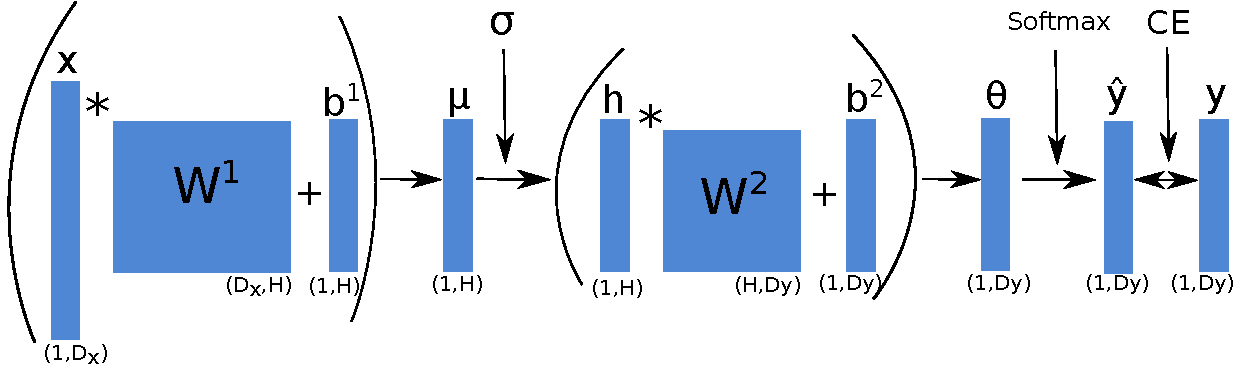
\includegraphics[scale=0.85]{neural.pdf}
\end{center}
\caption{A two layers neural network}
\label{neural}
\end{figure}
To be more formal, we can define all variables in the figure as:
 \begin{equation}\label{eq:1}
\mu_i = \sum_{s=1}^{D_{x}}W^{1}_{si} x_{s} + b^{1}_{i}  \; {\small \text{ with }i = 1, \dots, H}
\end{equation}
\begin{equation}\label{eq:2}
h_i = \sigma(\mu_i)  \; {\small \text{ with }i = 1, \dots, H}
\end{equation}
\begin{equation}\label{eq:3}
\theta_j = \sum_{s=1}^{H}W^{2}_{sj} h_{s} + b^{2}_{j} \;\; {\small \text{ with }j = 1, \dots, D_{y}}
\end{equation}
\begin{equation}\label{eq:4}
\hat{y}_j = softmax(\theta_j) \;\; {\small \text{ with }j = 1, \dots, D_{y}}
\end{equation}
\begin{equation}\label{eq:5}
J(y,\hat{y}) = CE(y,\hat{y}) = -\sum_{s=1}^{D_{y}} y_s  \log(\hat{y}_s)
\end{equation}
where CE stands for \textit{cross-entropy}. Let $k$ be the only index in ${1,\dots,D_{y}}$ such that $y_k =1$. So, equation (\ref{eq:5}) can be simplified as 

\begin{equation}\label{eq:6}
J(y,\hat{y}) = - \theta_k + \log(\sum_{j^{\prime}=1}^{D_{y}} e^{\theta_{j^{\prime}}})
\end{equation}

Now we will take all the relevant derivatives.\\

\textbf{2b)} First, for $j = 1, \dots, D_{y}$:
\begin{align*}
\frac{\partial J(y,\hat{y})}{\partial \theta_j}  & = \frac{\partial}{\partial \theta_j}(- \theta_k + \log(\sum_{j^{\prime}=1}^{n} e^{\theta_{j^{\prime}}})) \\
& = - \varphi_j + \frac{\partial}{\partial \theta_j}\log(\sum_{j^{\prime}=1}^{n} e^{\theta_{j^{\prime}}}) \\
& = - \varphi_j + \frac{1}{\sum_{j^{\prime}=1}^{n} e^{\theta_{j^{\prime}}}}\frac{\partial}{\partial \theta_j} e^{\theta_{j}} \\
& = - \varphi_j + \frac{e^{\theta_{j}}}{\sum_{j^{\prime}=1}^{n} e^{\theta_{j^{\prime}}}}\\
& = softmax(\theta_{j}) - \varphi_j \; ,
\end{align*}
where $\varphi_j = 1$ if $j=k$ and $\varphi_j = 0$ otherwise. Thus,
\[
\frac{\partial J(y,\hat{y})}{\partial \theta_j} = \hat{y}_{j} - y_{j} \; .
\]
For $ i \in {1,\dots,H}$ and $j \in {1,\dots,D_{y}}$ we have
\begin{align*}
\frac{\partial J(y,\hat{y})}{\partial W^{2}_{ij}}  & = \frac{\partial J(y,\hat{y})}{\partial \theta_j} \frac{\partial\theta_j}{\partial W^{2}_{ij}} \\
& = (\hat{y}_{j} - y_{j})h_{i}\; .
\end{align*}

For $j \in {1,\dots,D_{y}}$ we have
\begin{align*}
\frac{\partial J(y,\hat{y})}{\partial b^{2}_{j}}  & = \frac{\partial J(y,\hat{y})}{\partial \theta_j} \frac{\partial\theta_j}{\partial bW^{2}_{j}} \\
& = \hat{y}_{j} - y_{j}\; .
\end{align*}

For $ i \in {1,\dots,H}$ we have
\begin{align*}
\frac{\partial J(y,\hat{y})}{\partial h_{i}}  & =\sum_{j^{\prime} =1}^{D_{y}} \frac{\partial J(y,\hat{y})}{\partial \theta_{j^{\prime}}} \frac{\partial\theta_{j^{\prime}}}{\partial h_{i}} \\
& = \sum_{j^{\prime}=1}^{D_{y}}(\hat{y}_{j^{\prime}} - y_{j^{\prime}})W^{2}_{ij^{\prime}}\; .
\end{align*}

For simplicity sake, let $E_{i} := \sum_{j^{\prime}}^{D_{y}}(\hat{y}_{j^{\prime}} - y_{j^{\prime}})W^{2}_{ij^{\prime}}$. So, for $ i \in {1,\dots,H}$, 

\begin{align*}
\frac{\partial J(y,\hat{y})}{\partial \mu_{i}}  & =\frac{\partial J(y,\hat{y})}{\partial h_i} \frac{\partial h_i}{\partial \mu_{i}} \\
& = E_{i}\sigma^{\prime}(\mu_{i})\; .
\end{align*}

For $j \in {1,\dots,D_{x}}$  and $ i \in {1,\dots,H}$ we have
\begin{align*}
\frac{\partial J(y,\hat{y})}{\partial W^{1}_{ji}}  & = \frac{\partial J(y,\hat{y})}{\partial \mu_{i}} \frac{\partial\mu_{i}}{\partial  W^{1}_{ji}} \\
& =  E_{i}\sigma^{\prime}(\mu_{i})x_{j}\; .
\end{align*}

And for $ i \in {1,\dots,H}$ we have
\begin{align*}
\frac{\partial J(y,\hat{y})}{\partial b^{1}_{i}}  & = \frac{\partial J(y,\hat{y})}{\partial \mu_{i}} \frac{\partial\mu_{i}}{\partial  b^{1}_{i}} \\
& =  E_{i}\sigma^{\prime}(\mu_{i})\; .
\end{align*}

\textbf{2c)} Now, let $j \in {1,\dots,D_{x}}$ using the formulas above we can calculate the value of $\frac{\partial J(y,\hat{y})}{\partial x_{j}}$:
\begin{align*}
\frac{\partial J(y,\hat{y})}{\partial x_{j}}  & = \sum_{i=1}^{H}\frac{\partial J(y,\hat{y})}{\partial \mu_{i}} \frac{\partial\mu_{i}}{\partial  x_{j}} \\
& =  \sum_{i=1}^{H}E_{i}\sigma^{\prime}(\mu_{i})W^{1}_{ji}\; .
\end{align*}

\textbf{2d)} The number of parameters ($\# params$) can be calculate by the following equation:
\[
\# params = (D_{x}H) + (H D_{y}) + H + D_{y}
\]

\textbf{2e)}
\begin{minted}{python}
def sigmoid(x):
    # ## YOUR CODE HERE
    x = 1/(1 + np.exp(-x))
    # ## END YOUR CODE
    return x
    
def sigmoid_grad(f):
    # ## YOUR CODE HERE
    f = f*(1-f)
    # ## END YOUR CODE
    return f
\end{minted}

\textbf{2f)}

\begin{minted}{python}
def gradcheck_naive(f, x):
        # YOUR CODE HERE:
        x_plus_h = np.array(x, copy=True)
        x_plus_h[ix] = x_plus_h[ix] + h
        random.setstate(rndstate)
        fxh_plus, _ = f(x_plus_h)
        x_minus_h = np.array(x, copy=True)
        x_minus_h[ix] = x_minus_h[ix] - h
        random.setstate(rndstate)
        fxh_minus, _ = f(x_minus_h)
        numgrad = (fxh_plus - fxh_minus)/(2*h)
        # END YOUR CODE
\end{minted}

To implement the forward and back propagation, we need to consider the model represented in Figure \ref{neural} for every entry $(x^{1},y^{1}), \dots ,(x^{N},y^{N})$ of the dataset. Hence, we will have variables such as $x^{d},\mu^{d},h^{d},\theta^{d},\hat{y}^{d},y^{d},E^{d}$. And so the cost function and the gradients are:

\begin{equation}\label{eq:7}
Cost = \frac{1}{N}\sum_{d=1}^{N}J(y^{d},\hat{y}^{d})
\end{equation}

\begin{equation}\label{eq:8}
\frac{\partial Cost}{\partial W^{1}_{ji}} = \frac{1}{N}\sum_{d=1}^{N}E^{d}_{i}\sigma^{\prime}(\mu^{d}_{i})x^{d}_{j}
\end{equation}

\begin{equation}\label{eq:9}
\frac{\partial Cost}{\partial b^{1}_{i}} = \frac{1}{N}\sum_{d=1}^{N}E^{d}_{i}\sigma^{\prime}(\mu^{d}_{i})
\end{equation}

\begin{equation}\label{eq:10}
\frac{\partial Cost}{\partial W^{2}_{ij}} = \frac{1}{N}\sum_{d=1}^{N}(\hat{y}^{d}_{j} - y^{d}_{j})h^{d}_{i}
\end{equation}

\begin{equation}\label{eq:11}
\frac{\partial Cost}{\partial b^{2}_{j}} = \frac{1}{N}\sum_{d=1}^{N}(\hat{y}^{d}_{j} - y^{d}_{j})
\end{equation}



Remember, $E^{d}_{i} := \sum_{j^{\prime}}^{D_{y}}(\hat{y}^{d}_{j^{\prime}} - y^{d}_{j^{\prime}})W^{2}_{ij^{\prime}}$ for $ d \in {1,\dots,N}$ and $i \in {1,\dots,H}$. \\


\textbf{2g)} Equations (\ref{eq:7}) through (\ref{eq:11}) are the ones implemented in the following code (in vectorized form):

\begin{minted}{python}
def forward_backward_prop(data, labels, params, dimensions):
    # ## YOUR CODE HERE: forward propagation
    N = data.shape[0]
    all_mu = data.dot(W1) + b1
    all_h = sigmoid(all_mu)
    all_theta = all_h.dot(W2) + b2
    all_y_hat = softmax(all_theta)
    all_costs = np.sum(labels * np.log(all_y_hat), 1) * -1
    cost = np.mean(all_costs)
    # ## END YOUR CODE

    # ## YOUR CODE HERE: backward propagation
    subtraction = all_y_hat - labels
    E = np.dot(W2, subtraction.T)
    sig_mu = sigmoid_grad(sigmoid(all_mu.T))
    E_sig_mu_mult = E * sig_mu
    gradW1 = np.dot(data.T, E_sig_mu_mult.T) * 1/N
    gradb1 = np.sum(E_sig_mu_mult, 1) * 1/N
    gradW2 = np.dot(all_h.T, subtraction) * 1/N
    gradb2 = np.sum(subtraction.T, 1) * 1/N
    # ## END YOUR CODE
\end{minted}
\section{3}
Before we start let us set some notation. The vocabulary is composed of the following words $\{\wo_1, \dots ,\wo_W \}$. To make things simple we will represent every word $\wo_i$ by its index $i$. For $w \in \{1,\dots,W\}$ $y^{w}  \in \mathbb{R}^{W}$ is the one-hot vector such that $y^{w}_{w}=1$. $V = [v_1, \dots,v_W]$ is the matrix of all \textit{input vectors} and $U = [u_1, \dots,u_W]$ is the matrix of all \textit{output vectors}.

Given an input vector $v_c$ we can compute $\hat{y} \in \mathbb{R}^{W}$ as follows:
\[
\hat{y}_{o} = p(o|c) = \frac{exp(u_{o}^{T}v_{c})}{\sum_{w=1}^{W}exp(u_{w}^{T}v_{c})}
\]
where $exp(u_{o}^{T}v_{c})$ is just a different notation for $e^{u_{o}^{T}v_{c}}$. Now consider the following lost function:
\[
J_{softmax - CE}(o,v_c,U) = CE(y^{o},\hat{y})
\]

\textbf{3a)} For $ j \in {1,\dots,W}$
\begin{align*}
\frac{\partial J_{softmax - CE}(o,v_c,U)}{\partial v_{cj}}  & = \sum_{w=1}^{W}(\hat{y}_{w} = y^{o}_{w})u_{wj}\; .
\end{align*}

\textbf{3b)} For $ j \in {1,\dots,W}$
\begin{align*}
\frac{\partial J_{softmax - CE}(o,v_c,U)}{\partial u_{wj}}  & = v_{cj}(\hat{y}_{w} = y^{o}_{w})\; .
\end{align*}

\textbf{3c)} Let $[i_{1}, \dots, i_{K}]$ be the list of all $K$ sampled words (where $i_s \in \{1, \dots, W\}$). It should be noted that can be repetitions in this list, and $o \notin [i_{1}, \dots, i_{K}]$. The cost function associated is
\[
J_{neg - sample}(o,v_c,U) = - \log(\sigma(u_{o}^{T}v_{c})) - \sum_{k=1}^{K} \log(\sigma(-u_{i_{k}}^{T}v_{c}))
\]

For $ j \in {1,\dots,W}$
\begin{align*}
\frac{\partial J_{neg - sample}(o,v_c,U)}{\partial v_{cj}}  & = - \sigma(-u_{o}^{T}v_{c})u_{oj} - \sum_{k=1}^{K}\sigma(-u_{i_{k}}^{T}v_{c})u_{i_{k}j}
\end{align*}

\begin{align*}
\frac{\partial J_{neg - sample}(o,v_c,U)}{\partial u_{oj}}  & = - \sigma(-u_{o}^{T}v_{c})v_{cj}
\end{align*}

For $i_s \in \{i_{1}, \dots,i_{K}\}$,
\begin{align*}
\frac{\partial J_{neg - sample}(o,v_c,U)}{\partial u_{i_{s}j}}  & = - \#(i_s)\sigma(u_{i_{s}}^{T}v_{c})v_{cj}
\end{align*}

where $\#(i_s)$ is the number of times that $i_s$ occur in the list $[i_{1}, \dots, i_{K}]$.\\

Since we choose $K < W$, it is faster to compute $\sum_{k=1}^{K} \log(\sigma(-u_{i_{k}}^{T}v_{c}))$ than $\log(\sum_{w=1}^{W}exp(u_{w}^{T}v_{c}))$. The speed-up ration in this case is $\frac{W}{K}$.\\

\textbf{3d)} First let us deal with the \textbf{skipgram} model. $c$ is the center word and $[c-m, \dots,c-1, c+1, \dots,c+m]$ is the list of context words (here $m$ is the context size) - remember we are identifying the words with their indexes. Let $F(o,v)$ be a place holder for $J_{neg - sample}(o,v,U)$ and $J_{softmax - CE}(o,v,U)$. So the cost function of this model is
\[
J_{skipgram}(c-m, \dots,c,\dots, c+m) = \sum_{\substack{-m \leq j \leq m \\ j\neq 0}}F(c+j, v_c)
\]
Therefore, 
\begin{align*}
\frac{\partial J_{skipgram}}{\partial v_{c}}  & = \sum_{\substack{-m \leq j \leq m \\ j\neq 0}}\frac{\partial F(c+j,v_c)}{\partial v_{c}} 
\end{align*}

\begin{align*}
\frac{\partial J_{skipgram}}{\partial u_{w}}  & = \sum_{\substack{-m \leq j \leq m \\ j\neq 0}}\frac{\partial F(c+j,v_c)}{\partial u_{w}} 
\end{align*}

The \textbf{CBOW} model has a similar cost function:
\[
J_{CBOW}(c-m, \dots,c,\dots, c+m) = F(c, \hat{v})
\]
where 
\[
\hat{v} = \sum_{\substack{-m \leq j \leq m \\ j\neq 0}}v_{c+j}
\]
Thus,

\begin{align*}
\frac{\partial J_{CBOW}}{\partial u_{w}}  & = \frac{\partial F(c, \hat{v})}{\partial u_{w}} 
\end{align*}

\begin{align*}
\frac{\partial J_{CBOW}}{\partial u_{w}}  & = \frac{\partial F(c, \hat{v})}{\partial u_{w}} 
\end{align*}

\begin{align*}
\frac{\partial J_{CBOW}}{\partial v_{w}}  & = \#(w,[c-m, \dots,c-1, c+1, \dots,c+m])\frac{\partial F(c, \hat{v})}{\partial u_{w}} 
\end{align*}
where $\#(w,[c-m, \dots,c-1, c+1, \dots,c+m])$ is the frequency of the word $w$ in the list $[c-m, \dots,c-1, c+1, \dots,c+m]$.

\pagebreak

\textbf{3e)}
\begin{minted}{python}
def normalizeRows(x):
    # ## YOUR CODE HERE
    all_norm2 = np.sqrt(np.sum(np.power(x, 2), 1))
    all_norm2 = 1/all_norm2
    x = x * all_norm2[:, np.newaxis]
    # ## END YOUR CODE
    return x
    
def softmaxCostAndGradient(predicted, target, outputVectors, dataset):
    # ## YOUR CODE HERE
    y_hat = (softmax(outputVectors.dot(predicted))).flatten()
    y = np.zeros(outputVectors.shape[0])
    y[target] = 1
    cost = np.sum(y * np.log(y_hat)) * -1
    subtraction = y_hat - y
    gradPred = np.sum(subtraction*outputVectors.T, 1)
    grad = np.outer(subtraction, predicted)
    # ## END YOUR CODE
    return cost, gradPred, grad

def negSamplingCostAndGradient(predicted,
                               target,
                               outputVectors,
                               dataset,
                               K=10):
    # ## YOUR CODE HERE
    random_sample = []
    while len(random_sample) < K:
        pick_idx = dataset.sampleTokenIdx()
        if pick_idx != target:
            random_sample.append(pick_idx)
    sample_vectors = outputVectors[random_sample, :]
    target_pred = outputVectors[target].dot(predicted)
    sample_pred = sample_vectors.dot(predicted)
    cost = - (np.log(sigmoid(target_pred)) +
              np.sum(np.log(sigmoid(-sample_pred))))

    gradPred = - sigmoid(- target_pred)*outputVectors[target] + np.dot(
        sigmoid(sample_pred), sample_vectors)

    grad = np.zeros(outputVectors.shape)
    grad[target] = - sigmoid(- target_pred) * predicted
    counter = Counter(random_sample)
    for i in counter.keys():
        grad[i] = counter[i]*(sigmoid(outputVectors[i].dot(predicted)) *
                              predicted)
    # ## END YOUR CODE
    return cost, gradPred, grad


def skipgram(currentWord,
             C,
             contextWords,
             tokens,
             inputVectors,
             outputVectors,
             dataset,
             word2vecCostAndGradient=softmaxCostAndGradient):
    # ## YOUR CODE HERE
    current_index = tokens[currentWord]
    v_hat = inputVectors[current_index]
    cost = 0
    gradIn = np.zeros(inputVectors.shape)
    gradOut = np.zeros(outputVectors.shape)
    for word in contextWords:
        target = tokens[word]
        word_cost, word_gradPred, word_grad = word2vecCostAndGradient(v_hat,
                                                                      target,
                                                                      outputVectors,
                                                                      dataset)
        cost += word_cost
        gradIn[current_index] += word_gradPred
        gradOut += word_grad
    # ## END YOUR CODE
    return cost, gradIn, gradOut
\end{minted}

\pagebreak

\textbf{3g)} As we can see in Figure \ref{word_vectors} words with similar meaning are close together like amazing and annoying, cool and boring, well and good. Punctuation symbols as ! and ? are close from each other and distant from other words. The same apply for articles the and a.  \\

\begin{figure}
\begin{center}
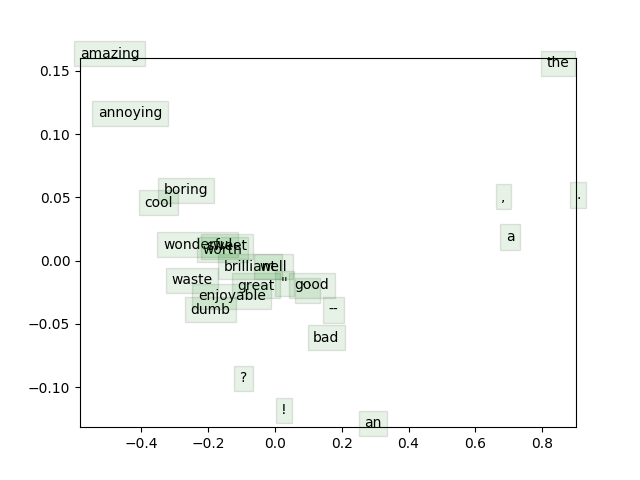
\includegraphics[scale=0.85]{q3_word_vectors.png}
\end{center}
\caption{A visualization of the word vectors}
\label{word_vectors}
\end{figure}

\textbf{3h)}
\begin{minted}{python}
def cbow(currentWord,
         C,
         contextWords,
         tokens,
         inputVectors,
         outputVectors,
         dataset,
         word2vecCostAndGradient=softmaxCostAndGradient):
    # ## YOUR CODE HERE
    gradIn = np.zeros(inputVectors.shape)
    current_index = tokens[currentWord]
    context_indexes = [tokens[word] for word in contextWords]
    v_hat = np.sum(inputVectors[context_indexes], axis=0)
    cost, input_vector_grad, gradOut = word2vecCostAndGradient(v_hat,
                                                               current_index,
                                                               outputVectors,
                                                               dataset)
    counter = Counter(context_indexes)
    for i in counter.keys():
        gradIn[i] = counter[i]*input_vector_grad
    # ## END YOUR CODE
    return cost, gradIn, gradOut
\end{minted}

\section{4}

As in the case of the neural network, let us take a look in the multinomial logistic regression model. In this case we have a dataset of the form $(x^{1},y^{1}) \dots ,(x^{N},y^{N})$ where each $x^{d} \in \mathbb{R}^{n}$ is a vector of features and $y^{d} \in\{1, \dots, K\}$ ($K$ is the number of classes). Let $W \in \mathbb{R}^{n,K}$, for $i \in\{1, \dots, K\}$  we define:
\[
\hat{y}(W,x)_{i} = softmax(\sum_{s=1}^{n}W_{si}x_{s})
\]
Let $hot(y) \in \mathbb{R}^{K}$ be the one-hot vector representation of $y$, i.e., $hot(y)_{i} = 1$ iff $y=i$. We call $\lambda \in \mathbb{R}$ a regularization parameter and use it to define the cost function of the model:
\[
J(W) = \frac{1}{N}\sum_{d=1}^{N}(CE(hot(y^{d}),\hat{y}(W,x^{d}))  + \frac{1}{2}\lambda\sum_{i=1}^{n}\sum_{j=1}^{K} (W_{ij})^{2})
\]
Hence, for $i \in\{1, \dots, n\}$ and $j \in\{1, \dots, K\}$
\[
\frac{\partial J(W)}{\partial W_{ij}} = \frac{1}{N}\sum_{d=1}^{N}x^{d}_{i}(\hat{y}(W,x^{d})_{j} - hot(y^{d})_{j})  + \lambda W_{ij}
\]



\textbf{4a)}
\begin{minted}{python}
def getSentenceFeature(tokens, wordVectors, sentence):

    # ## YOUR CODE HERE
    sentence_tokens = [tokens[word] for word in sentence]
    size_factor = 1.0/len(sentence)
    sentVector = size_factor * np.sum(wordVectors[sentence_tokens], axis=0)
    # ## END YOUR CODE
    return sentVector

def softmaxRegression(features,
                      labels,
                      weights,
                      regularization=0.0,
                      nopredictions=False):
    prob = softmax(features.dot(weights))
    if len(features.shape) > 1:
        N = features.shape[0]
    else:
        N = 1
    # A vectorized implementation of
    # 1/N * sum(cross_entropy(x_i, y_i)) + 1/2*|w|^2
    cost = np.sum(-np.log(prob[range(N), labels])) / N
    cost += 0.5 * regularization * np.sum(weights ** 2)

    # ## YOUR CODE HERE: compute the gradients and predictions
    num_classes = weights.shape[1]
    all_one_hot = np.zeros((N, num_classes))
    all_one_hot[np.arange(len(labels)), labels] = 1
    subtraction = prob - all_one_hot
    grad = (np.dot(features.T, subtraction) / N) + (weights * regularization)
    pred = np.argmax(prob, axis=1)
    # ## END YOUR CODE

    if nopredictions:
        return cost, grad
    else:
        return cost, grad, pred
\end{minted}

\textbf{4b)} Since $W$ appear in the cost function, after the minimization  each value of $W$ will be small. Small values for the parameters will correspond to a simpler hypothesis, thus preventing overfitting. \\

\textbf{4c)}
\begin{minted}{python}
# ## YOUR CODE HERE
reg_minus2 = np.random.random_sample([10]) / 10
reg_minus3 = np.random.random_sample([10]) / 100
reg_minus4 = np.random.random_sample([10]) / 1000
reg_minus5 = np.random.random_sample([10]) / 10000
reg_minus6 = np.random.random_sample([10]) / 100000
REGULARIZATION = np.concatenate((reg_minus2,
                                 reg_minus3,
                                 reg_minus4,
                                 reg_minus5,
                                 reg_minus6))
REGULARIZATION.sort()
print("All the regularization params are = {}".format(REGULARIZATION))
# ## END YOUR CODE

# ## YOUR CODE HERE
best_result = - float('inf')
for i in range(len(results)):
    if results[i]["dev"] > best_result:
        best_result = results[i]["dev"]
        BEST_REGULARIZATION = results[i]["reg"]
        BEST_WEIGHTS = results[i]["weights"]

# ## END YOUR CODE
\end{minted}

Since we do not have any information for $\lambda$ we start with 50 random values for it (all in the interval $(0,1)$) with different orders of magnitude. The following table show the results for the selected value.

\begin{center}
\begin{tabular}{|c|c|c|c|}
\hline
\rowcolor{blue!20}
Regularization parameter & Train accuracy ($\%$) & Dev accuracy ($\%$) & Test accuracy ($\%$)\\ \hline
$7.416922 \times 10^{-5}$ & $29.541199$ & $30.426885$ & $28.144796$\\ \hline
\end{tabular}
\end{center}

\pagebreak

\textbf{4d)} Figure \ref{results} shows that as long as the regularization parameter $\lambda$ get bigger there is a decay in accuracy both in the train dataset as in the dev dataset. In the interval around $10^{-4}$ the parameter provides a reasonable generalization, i.e., the accuracy in the dev dataset is better than in the train dataset.
\begin{figure}
\begin{center}
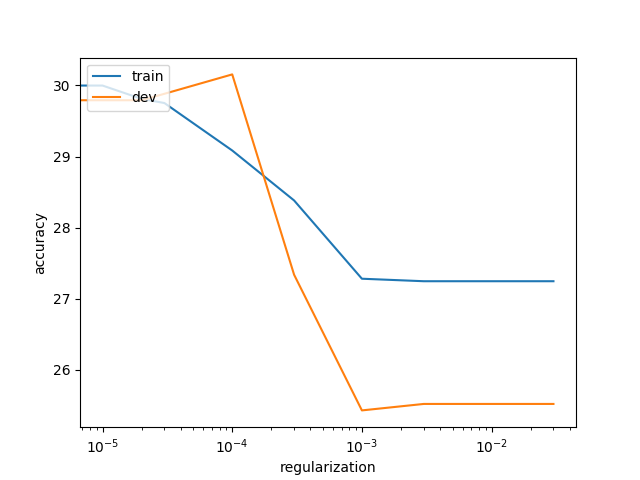
\includegraphics[scale=1]{q4_reg_v_acc.png}
\end{center}
\caption{Classification accuracy}
\label{results}
\end{figure}





\end{document}
